\documentclass{article}
\usepackage{amssymb,amsmath}
\usepackage{mathtools}
\usepackage{array}
\usepackage{color}
\usepackage{graphicx}
\usepackage{minted}
% \pagecolor{black}
% \color{white}
\topmargin=-0.3in
\textheight=9.2in
\textwidth=168mm
\oddsidemargin=-0.2in
\evensidemargin=-0.2in

\newcommand{\sqr}{$\square \qquad|$ & $\square \qquad|$ & $>\qquad|$ & $\square\qquad|$ & $\square\ \qquad$ }

\title{Computer Organization Exam Review}
\date{}

\begin{document}
\maketitle
\begin{enumerate}
\item $CPU\ Time = \frac{Clock\ Cycles}{Clock\ Rate}$
\item $CPU\ Time = Instructions \times \frac{Cycles}{Instruction} \times \frac{Seconds}{Cycle}$
\item $CPU\ Time = Clock\ Cycles \times Cycle\ Time$
\item $CPI = \frac{Clock\ Cycles}{Instructions}$
\item $CPU\ Time = Instruction\ Count \times CPI \times Cycle\ Time$
\item $CPU\ Time = Instruction\ Count \times \frac{CPI}{Clock\ Rate}$
\item $(Clock\ Cycles)_{Total} = \sum_{i = 1}^{n}\left(CPI_{i} \times Count_{i}\right)$
\item $MIPS = \frac{Instruction\ Count}{CPU\ Time \times 10^{6}}$
\item $Power = Capacitive\ Load \times (Voltage)^{2} \times Frequency$
\item $AMAT = Hit\ Time + Miss\ Rate \times Miss\ Penalty$
\end{enumerate}
\hrule
\begin{enumerate}
\item Identify the data hazards in the following code, and fix them using $nop$ (software).
\begin{center}
\begin{minted}[linenos=true]{nasm}
sub $2, $1, $3
and $12, $2, $5
or  $13, $6, $2
add $14, $2, $2
sw  $15, 100($2)
\end{minted}
\end{center}
\indent The data hazard is present in the $\$2$ register.
The $sub$ instruction will take three cycles to write to the $\$2$ register, but the $and$ and $or$ instructions are attempting to access $\$2$ before the register has a value in it.
As a result, two $nop$ instructions should be inserted after the $sub$ instruction to offset the data access.
\begin{minted}[linenos=true]{nasm}
sub $2, $1, $3
nop
nop
and $12, $2, $5
or  $13, $6, $2
add $14, $2, $2
sw  $15, 100($2)
\end{minted}
\item Identify and fix the data hazards shown below by showing the fowarding paths (hardware).
\begin{minted}[linenos=true]{nasm}
add $3, $4, $6
sub $5, $3, $2
lw  $7, 100($5)
%add $8, $7, $2
\end{minted}
There are two data hazards in this set of instructions.
In line two, register $\$3$ is being accessed by the $sub$ instruction before it is stored by the $add$ instruction.
The other hazard is with the $\$7$ register, which is used by the $add$ instruction before a value is loaded by the $lw$ instruction.\\
% \begin{tabular}{l c c c c c c c c c}
% $add$ & \sqr & & & &\\
% $sub$ & & \sqr & & &\\
% $lw$  & & & \sqr & &\\
% $nop$ & & & & \sqr &\\
% $add$ & & & &  &\sqr\\
% \end{tabular}
\item Compare the performance for the single-cycle, multi-cycle, and piplined control using the following instruction mix.
\begin{center}
\begin{tabular}{|l|c|c|c|c|c|}
\hline
& Loads & Stores & Branches & Jumps & ALU\\
\hline
Instruction Mix & 25\% & 10\% & 11\% & 2\% & 52\%\\
\hline
Clock Cycles & 5 & 4 & 3 & 3 & 4\\
\hline
\end{tabular}
\end{center}
The performance for a single cycle machine is 200ps for memory access, 100ps for ALU operations, and 50ps for register read and write.
In a piplined implementation, loads, stores, and ALU operations take 1 clock cycle.
Branches take 1 clock cycle when predicted correctly, and 2 when not;
Jumps take 2 clock cycles.
\begin{enumerate}
\item What is the clock cycle time for a single-cycle data path?\\
\indent In order calculate the clock cycle time, we need to know how long each instruction takes to execute.
We can create the following table to calculate the total time:\\

\hspace*{-1.7cm}
\begin{tabular}{|c|c|c|c|c|c|c|}
\hline
Instruction Class & Instruction Memory & Register Read & ALU Op & Data Memory & Register Write & Total\\
\hline
R-Type & 200 & 50 & 100 & 0 & 50 & 400\\
\hline
Load Word & 200 & 50 & 100 & 200 & 50 & 600\\
\hline
Store Word & 200 & 50 & 100 & 200 & 0 & 550\\
\hline
Branch & 200 & 50 & 100 & 0 & 0 & 350\\
\hline
Jump & 200 & 0 & 0 & 0 & 0 & 200\\
\hline
\end{tabular}
\vspace{0.1cm}

The single cycle implementation is bottlenecked by the longest instruction, which happens to be the Load Word instruction.
Therefore, the clock cycle time is 600ps.
\item What is the average CPI for the multi-cycle design?\\
\indent The CPI for the multi-cycle design is dependant on the number of types of instruction that appear in the program.
To calculate the CPI, we have
\begin{align*}
CPI &= (0.25)(5) + (0.1)(4) + (0.11)(3) + (0.02)(3) + (0.52)(4)\\
&= 4.12\ \text{cycles per instruction}
\end{align*}
\item What is the average CPI for the piplined design?\\
\indent The pipelined design's CPI, like the multi-cycle, is determined by the number of types of instructions that appear in the program.
However, the piplined cycle uses less clock cycles per instruction in this implementation.
In addition, the branch instructions have a $50\%$ of being correct, so we need to find the average clock cycle time for the branches.
We can find the CPI for the pipelined design as follows:
\begin{align*}
CPI &= (0.25)(1) + (0.1)(1) + (0.11)\left(\frac{1 + 2}{2}\right) + (0.02)(2) + (0.52)(1)\\
&= 1.075\ \text{cycles per instruction}
\end{align*}
\item What are the average instruction times for each designs?\\
The single cycle datapath's instruction time is determined by the longest instruction time, which is the 600ps load word.
The multicycle and pipelined datapath are dependant on the longest clock cycle in the longest instruction, which is 200ps.
We then tak that and multiply it by the CPI, which yields 824ps for the multicycle datapath, and 215ps for the pipelined datapath.
\end{enumerate}
\item Assume an instruction cache miss rate for a program is 2\% and a data cache miss rate is 4\%.
If the processor has a CPI of 2 without any memory stalls and the miss penalty of 100 cycles for all misses, determine how much faster a processor with a perfect cache that never misses would be.
The frequency of all loads and stores is 36\% for the SPECint2000.\\
\indent We will start by letting the instruction count $= \mathcal{I}$.
We know how to calculate the number of memory miss cycles:
\[
\mathcal{I}\times 0.02\times 100\text{ cycles} = 2\mathcal{I}.
\]
This result follows from the fact that the \textbf{cache} miss rate is 2\% with a penalty of 100 clock cycles.
We now need to calculate the number of memory miss cycles for data references.
Again, we know the frequency an penalty for \textbf{data cache} misses:
\[
\mathcal{I}\times 0.04\times 0.36\times 100 = 1.44\mathcal{I}.
\]
As a result, the total number of misses is $1.44\mathcal{I} + 2\mathcal{I}$, or $3.44\mathcal{I}$.
To obtain the CPI with stalls, we simply add the number of misses divided by the instruction count to the perfect CPI.
\[
\text{CPI}_{\text{Misses}} = 3.44 + 2 = 5.44.
\]
The ratio of the imperfect cache to the perfect cache is
\[
\frac{5.44}{2} = 2.72,
\]
so the perfect cache is 2.72 times faster than the imperfect cache.
\item For the following cache, answer the following questions.
\begin{center}
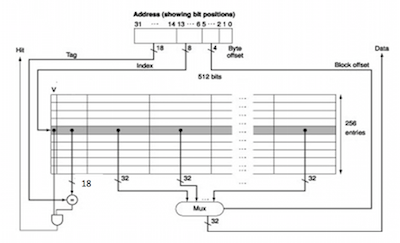
\includegraphics[scale=0.7]{hw5_graphic}
\end{center}
\begin{enumerate}
\item Compute the total size of the cache.\\
If we had not been given the number of entries in the cache, we could compute it as $2^{\text{index}}$, which is $2^{8}$, or $256$ in this case.
Each entry in the cache occupies 512 bits of memory, so the total size of the cache is $256 * 512 = 131072$.
\item Compute the total number of bits required to implement this cache for the Intrinsity FastMATH embedded microprocessor.\\
The total number of bits needed is determined by the total size of each entry in the cache.
There are 512 bits of memory in each entry, but there is also a 1 bit data entry and an 18 bit tag, which means each entry in the cache is $512 + 1 + 18 = 531$ bits.
With 256 entries, we have $531 * 256 = 135936$ bits.
\end{enumerate}
\item Consider a memory hierarchy using one of the three organizations for main memory shown below.
Assume that the cache block size is 16 words, that the width of organization (b) of the figure is four words,
and that the number of banks in organization (b) of the figure is four.
If the main memory latency for a new access is 10 memory bus clock cycles and the transfer time is 1 memory bus clock cycle, what are the miss penalties (in clock cycles) for each of these organizations?
\begin{center}
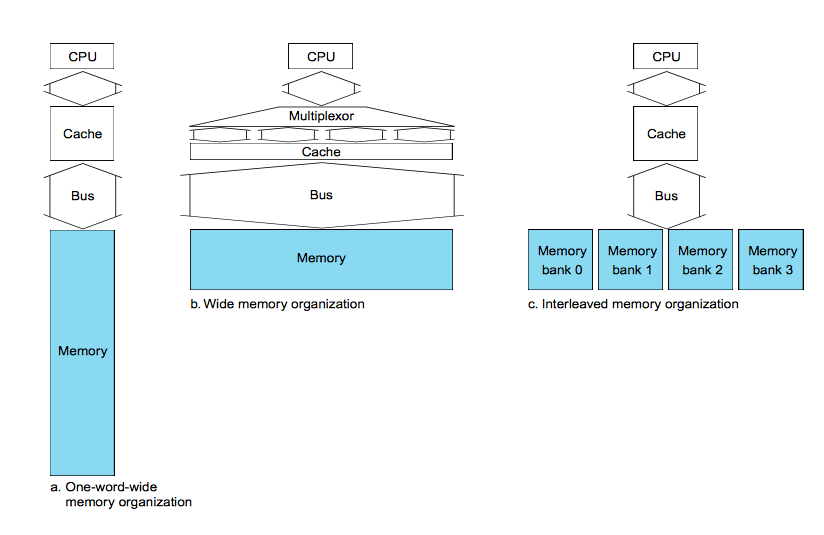
\includegraphics[scale=0.5]{hw5_graphic2}
\end{center}
\begin{enumerate}
\item For each organization, we will always have to go through the bus to access memory.
We know that we only have a miss if we have to move from the cache into memory and return the fetched memory back to the CPU.
For this particular computer, it takes 10 clock cycles to retrieve the memory.
As a result, we will have the following time for a miss penalty in the cache
\[
\text{Miss} = 1 + (10)(16) + (16)(1) = 177.
\]
\item For this organization, we have changed the amount of memory we have to search through; specifically, we now only need to access a quarter of the amount of memory that we have had to in (a).
We do still have to go though the bus, so we have
\[
\text{Miss} = 1 + (10)\left(\frac{16}{4}\right) + \left(\frac{16}{4}\right)(1) = 45.
\]
\item Finally, in this organization our memory has been split into four separate cells.
We still have to travese through the bus, so we know that we will have to wait the usual clock cycle.
Similar to (b), we will have to only search through a quarter of the memory to find the address that we need; we will however still have to transmit 16 words through the bus back to the cache.
This setup yields
\[
\text{Miss} = 1 + (10)\left(\frac{16}{4}\right) + (16)(1) = 57.
\]
\end{enumerate}
\item For the following diagram, explain what happens in each block for the instruction $lw\ \$t3, 100(\$t2)$.
\begin{center}
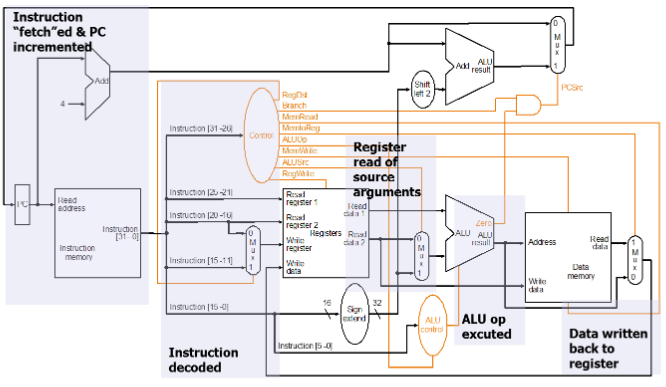
\includegraphics[scale=0.5]{review_01}
\end{center}
\begin{itemize}
\item \underline{Instruction Fetch:} The machine gathers the next instruction as determined by the program counter.
The PC increments by 4 every cycle, assuming the program does not encouter any exceptions or errors.
\item \underline{Instruction Decode:} In this step, the instruction is interpreted by the machine to be the load word instruction.
\item \underline{Register Read:} The appropriate registers are parsed, and the address is decoded.
\item \underline{ALU Operation:} The ALU adds the offest to the base address, and requests the contents of that location in memory.
\item \underline {Register Write:} The machine now writes the contents of memory that have been fetched to the $\$t3$ register.
\item \underline {Instruction Fetch:} The PC is incremented by 4, and the process continues for the next instruction.
\end{itemize}
% \item A compiler designer is trying to decide between two code sequences for a particular machine.
% Based on the hardware implementation, we have the following:
% \begin{center}
% \begin{tabular}{|l|c|c|c|}
% \hline
% Class & A & B & C\\
% \hline
% CPI & 1 & 2 & 3\\
% \hline
% \end{tabular}
% \end{center}
% The first code sequence has 5 instructions:
% 2 of A, 1 of B, and 2 of C.
% The second code sequence has 6 instruction:
% 4 of A, 1 of B, and 1 of C.
% \begin{enumerate}
% \item What is the CPI for each sequence?\\
% The CPI for the first sequence is
% \[
% 2 * 1 + 1 * 2 + 2 * 3 = 10.
% \]
% The CPI for the second sequence is
% \[
% 4 * 1 + 1 * 2 + 1 * 3 = 9.
% \]
% \item Which sequence is faster, and by how much?
%
% \end{enumerate}
\end{enumerate}
\end{document}
